\documentclass[12pt]{article}
\usepackage{lscape, xcolor}
\usepackage{verbatim}
\usepackage{amsmath,amsthm,amssymb}
\usepackage{colonequals,color,multirow}
\usepackage{enumerate}
\usepackage[sc]{mathpazo} % Use the Palatino font
\usepackage[T1]{fontenc} % Use 8-bit encoding that has 256 glyphs
\usepackage{times}	
% \usepackage{apacite}
\usepackage[authoryear]{natbib}
\usepackage[demo]{graphicx}
\usepackage{subcaption}
\usepackage{lscape, xcolor}
\usepackage{verbatim}
\usepackage{amsmath,amsthm,amssymb}
\usepackage[sc]{mathpazo} % Use the Palatino font
\usepackage[T1]{fontenc} % Use 8-bit encoding that has 256 glyphs
\usepackage{times}	
\usepackage{booktabs}
\usepackage{ caption, float}
\usepackage{enumitem}
\usepackage[left=1in, right=1in, top=1in, bottom=1in]{geometry}
\usepackage{blindtext}
\usepackage{titlesec}
\usepackage{graphicx}
%\graphicspath{/home/evo/4m_final_project}
\setcounter{secnumdepth}{4}
\usepackage{caption} % For subfigures with captions
\usepackage{subcaption} % For subfigures with captions
\captionsetup[subfigure]{labelformat=empty} % Removes the (a), (b) labels
\usepackage{hyperref}
\usepackage[authoryear]{natbib}
\titleformat{\paragraph}
{\normalfont\normalsize\bfseries}{\theparagraph}{1em}{}
\titlespacing*{\paragraph}
{0pt}{3.25ex plus 1ex minus .2ex}{1.5ex plus .2ex}
\renewcommand{\baselinestretch}{1.5}% Line spacing - Palatino needs more space 
\vspace{\baselineskip}
\linespread{1.5}




\begin{document}

\title{STATS 4M03: Multivariate Analysis\\ Final Project \\ Diabetes Dataset }

\author{Submitted to\\ Dr. Eman M.S. Alamer 
\\Department of Mathematics and Statistics
\\McMaster University\\Hamiltion, Ontario, Canada L8S 4K1}
\date {November 22, 2024}


\maketitle

 \centerline{Reported by}
 \centerline{Xinyi Chen (400326045)}
  \centerline{Tonu Xu(400370837)}
   \centerline{Rayyan Kazim(Student ID)}
    \centerline{Safi Khan (400402095)}
     \centerline{First last (Student ID)}


\newpage
%\thispagestyle{fancy} % All pages have headers and footers
\section{Introduction}
\subsection{Abstract}

The study of diabetes is vital in understanding the progression of the disease and identifying key predictors. Throughout this paper, we perform data analysis on the diabetes dataset, and will primarily focus on leveraging various statistical methods that we learned in STATS 4M03$\backslash$6M03: Multivariate Analysis. By using a variety of methods, our goal is to predict the onset of diabetes from detailed medical diagnostic measurements based on several contributing health factors, with the aim of uncovering patterns and relationships between various clinical and lifestyle factors. \\



The analysis begins with summarizing the dataset to gain insights into distributions, central tendencies, and variances of key variables such as blood glucose levels, BMI, and insulin levels. Correlation analysis highlights interdependencies among factors, while hypothesis testing identifies statistically significant differences between diabetic and non-diabetic populations. Regression models, including linear and logistic regression, are utilized to predict outcomes and assess risk factors like age, family history, and lifestyle habits.

This study aims to contribute to a deeper understanding of diabetes etiology and progression, emphasizing actionable insights for clinical decision-making and preventive strategies. The findings underscore the importance of statistical analysis in uncovering hidden trends and improving the accuracy of diabetes diagnosis and management. Future work may incorporate machine learning techniques for enhanced predictive modeling and broader applications in healthcare analytics.

............
\subsection{The Data}

In this paper, we will study the diabetes dataset. \cite{Kaggles} which can be found here: \href{https://www.kaggle.com/datasets/hasibur013/diabetes-dataset}{Diabetes Dataset}

The diabetes dataset contains 768 rows x 9 columns, representing various health diagnostic metrics for predicting diabetes. Each row corresponds to a unique patient record, with features capturing key medical attributes. Table 1 showcases each of the columns in the dataset and a description of each of the columns.

We will be using R \cite{Rlang} as our main computing software

\begin{table}[h!]
	\centering
	\resizebox{\textwidth}{!}{ % Resize to fit the width of the page
	\begin{tabular}{|c|c|}
		\hline
		\textbf{Column} & \textbf{Description Of Column} \\ \hline
		Pregnancies & Integer: Number of times the patient has been pregnant. \\ \hline
		Glucose & Integer: Plasma glucose concentration (mg/dL) after a 2-hour oral glucose tolerance test. \\ \hline
		BloodPressure & Integer: Diastolic blood pressure (mm Hg). \\ \hline
		SkinThickness & Integer: Triceps skinfold thickness (mm). \\ \hline
		Insulin & Integer: 2-hour serum insulin (mu U/ml). \\ \hline
		BMI  & Float: Body mass index, defined as weight in kg/(height in m)\^2. \\ \hline
		DiabetesPedigreeFunction & Float: A score indicating genetic predisposition to diabetes based on family history. \\ \hline
		Age & Integer: Age of the patient (in years). \\ \hline
		Outcome & Binary: Target variable where 1 indicates diabetes, and 0 indicates no diabetes. \\ \hline
	\end{tabular}
}
	\caption{Description of the Diabetes Dataset}
\end{table}

.......

\subsubsection{Exploratory Data Analysis (EDA)}
In this paper, we used several EDA methods to analyze our dataset. These methods include: PCA \cite{kurita2019principal}, and a normal QQ-plot \cite{marden2004positions}. some text \cite{Lecture2}
\paragraph{PCA}

From figure 1, we observe that we should take 3 principle components.

% \begin{figure}[h!]
%      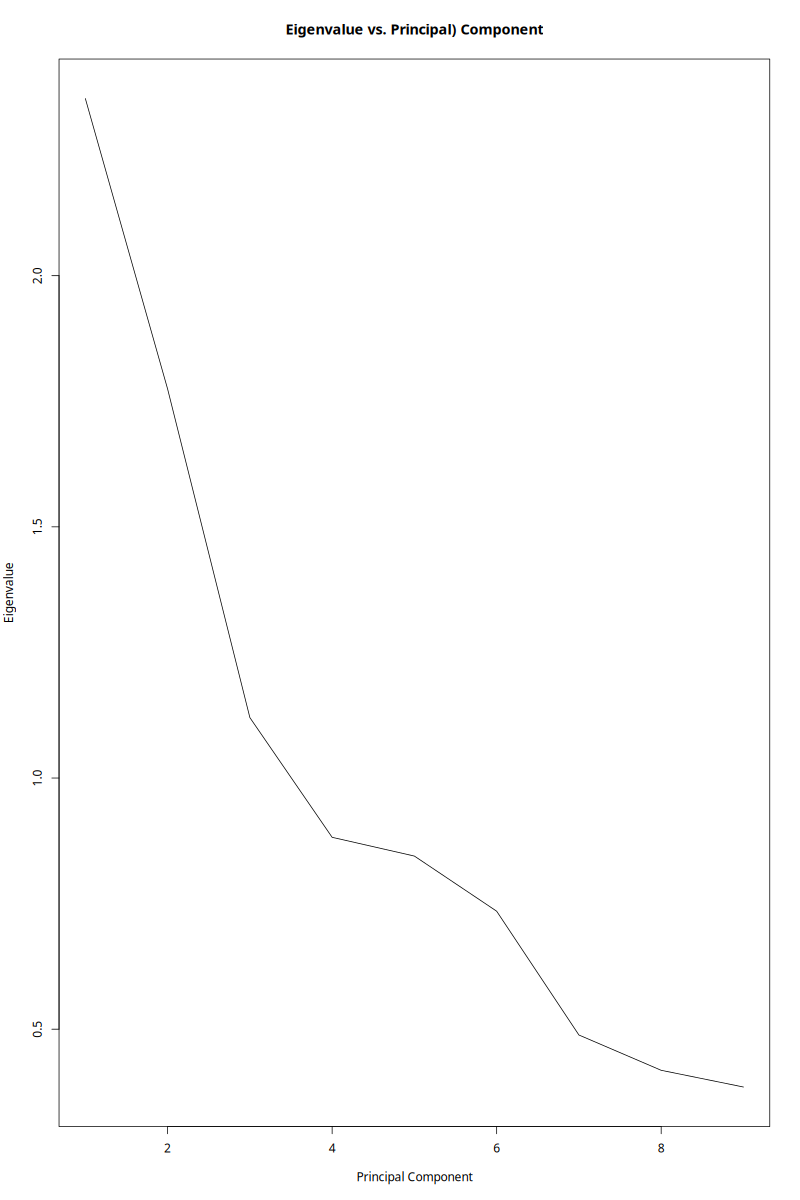
\includegraphics[width= 0.60\textwidth, height = 65mm]{eigenvalues_plot.png}\\
%     \caption{Plot of the eigenvalues}
% \end{figure}


\paragraph{QQ-plot}

From figure 2, we observe that the dataset is not normal


.......
\subsubsection{Data Preparation} 

We write about the training and testing here, and how we used column 9 as a label. We also scaled the dataset.\\

\section{Methodology}
\subsection{Supervised learning Analysis} 
 In this section, we perform supervised learning analysis using Classification trees: k-Nearest Neighbours and the following ensembles method: Random Forests Classifiers.\cite{zhou2012ensemble}
 
 \subsubsection{k-Nearest Neighbours}

 Firstly, we executed the k-Nearest Neighbours algorithm \cite{peterson2009k} on our dataset. The algorithm is a non-parametric, supervised learning classifier that uses proximity to make classifications about the grouping of a dataset.

 \subsubsection{Random Forest Classifiers}
 
 Also, we used the Random Forest Classifiers \cite{zhou2012ensemble} on our dataset. Random Forest classifiers is a bootstrapping sampling method that combines the results of multiple decision trees to draw on a conclusion. The algorithm \cite{Lecture16} is an extension of the bagging algorithm \cite{Lecture16} that creates uncorrelated decision trees, for each tree, a random sample of $\mathcal{M}$ is taken at each decision tree split.

\subsection{Binary Logistic Regression}
We performed a binary logistic regression analysis \cite{faraway2016extending}, a supervised learning method, to explore the relationship between various predictor variables and the binary response variable “Outcome,” indicating the presence or absence of diabetes. The initial model incorporated eight predictor variables: Pregnancies, Glucose, Blood Pressure, Skin Thickness, Insulin, BMI, Diabetes Pedigree Function, and Age. These variables were selected based on their potential relevance to diabetes risk, informed by existing domain knowledge.\\
\setlength{\parindent}{0pt}
The objective of the analysis was to identify the most significant predictors using the backward elimination method, a stepwise regression technique. This approach began with a model including all predictors, subsequently removing variables in sequence based on the highest p-value exceeding 0.05. This systematic elimination of statistically insignificant predictors not only enhances the model’s interpretability but also minimizes the risk of overfitting, ensuring that the final model retains only variables with significant contributions to predicting the outcome.

\subsection{Boosting}

Boosting \cite{chen2015xgboost} \cite{friedman2001greedy} is an ensemble learning technique that combines multiple weak learners, typically decision trees, to create a strong predictive model. For this analysis, we used XGBoost (Extreme Gradient Boosting), which is efficient and optimized for large datasets, to predict the presence of diabetes based on clinical measurements.

The model was trained on 70\% of the data, leaving 30\% for testing. The binary outcome variable (1 = diabetes, 0 = no diabetes) was predicted using features such as glucose levels, BMI, and age. Missing or zero values were present in some predictors (e.g., insulin), which could influence the model's performance.

\textbf{Model Parameters}
\begin{itemize}
	\item Learning rate (\texttt{eta}): 0.1
	\item Maximum tree depth (\texttt{max\_depth}): 6
	\item Evaluation metric: Area Under the Curve (AUC)
	\item Number of boosting rounds (\texttt{nrounds}): 100
\end{itemize}

\section{Discussion}
\subsection{Binary Logistic Regression}
\begin{table}[H]
\centering
\resizebox{\textwidth}{!}{ % Resize to fit the width of the page
\begin{tabular}{llllllll}
\cline{1-5}
\multicolumn{1}{|l|}{Coefficients:}             & \multicolumn{1}{l|}{Estimate}   & \multicolumn{1}{l|}{Std. Error} & \multicolumn{1}{l|}{z value} & \multicolumn{1}{l|}{Pr(\textgreater{}|z|)} &  &  &  \\ \cline{1-5}
\multicolumn{1}{|l|}{(Intercept)}              & \multicolumn{1}{l|}{-8.4398695} & \multicolumn{1}{l|}{0.8176393}  & \multicolumn{1}{l|}{-10.322} & \multicolumn{1}{l|}{\textless 2e-16}       &  &  &  \\ \cline{1-5}
\multicolumn{1}{|l|}{Pregnancies}              & \multicolumn{1}{l|}{0.1135092}  & \multicolumn{1}{l|}{0.0375672}  & \multicolumn{1}{l|}{3.021}   & \multicolumn{1}{l|}{0.00252}               &  &  &  \\ \cline{1-5}
\multicolumn{1}{|l|}{Glucose}                  & \multicolumn{1}{l|}{0.0343876}  & \multicolumn{1}{l|}{0.0042392}  & \multicolumn{1}{l|}{8.112}   & \multicolumn{1}{l|}{4.99E-16}              &  &  &  \\ \cline{1-5}
\multicolumn{1}{|l|}{BloodPressure}            & \multicolumn{1}{l|}{-0.0134342} & \multicolumn{1}{l|}{0.0059047}  & \multicolumn{1}{l|}{-2.275}  & \multicolumn{1}{l|}{0.0229}                &  &  &  \\ \cline{1-5}
\multicolumn{1}{|l|}{SkinThickness}            & \multicolumn{1}{l|}{0.0098866}  & \multicolumn{1}{l|}{0.0083722}  & \multicolumn{1}{l|}{1.181}   & \multicolumn{1}{l|}{0.23765}               &  &  &  \\ \cline{1-5}
\multicolumn{1}{|l|}{Insulin}                  & \multicolumn{1}{l|}{-0.0015283} & \multicolumn{1}{l|}{0.0009882}  & \multicolumn{1}{l|}{-1.546}  & \multicolumn{1}{l|}{0.122}                 &  &  &  \\ \cline{1-5}
\multicolumn{1}{|l|}{BMI}                      & \multicolumn{1}{l|}{0.0776662}  & \multicolumn{1}{l|}{0.0174657}  & \multicolumn{1}{l|}{4.447}   & \multicolumn{1}{l|}{8.72E-06}              &  &  &  \\ \cline{1-5}
\multicolumn{1}{|l|}{DiabetesPedigreeFunction} & \multicolumn{1}{l|}{0.8088779}  & \multicolumn{1}{l|}{0.332009}   & \multicolumn{1}{l|}{2.436}   & \multicolumn{1}{l|}{0.01484}               &  &  &  \\ \cline{1-5}
\multicolumn{1}{|l|}{Age}                      & \multicolumn{1}{l|}{0.0297298}  & \multicolumn{1}{l|}{0.0109345}  & \multicolumn{1}{l|}{2.719}   & \multicolumn{1}{l|}{0.00655}               &  &  &  \\ \cline{1-5}
\end{tabular}
}
\caption{Binary Logistic Regression }
\end{table}
From Table 2, the coefficient for “SkinThickness” had the highest p-value (0.23765 > 0.05), indicating it was not significantly associated with the outcome. At this stage, the misclassification rate was 0.22396. Consequently, “SkinThickness” was removed from the model. After removing “SkinThickness,” the coefficient for “Insulin” had the highest p-value (0.24334 > 0.05), indicating it was also not significant. Then 'insulin' was excluded from the model.\\
\begin{table}[H]
\centering
\resizebox{\textwidth}{!}{ % Resize to fit the width of the page
\begin{tabular}{llllllll}
\cline{1-5}
\multicolumn{1}{|l|}{Coefficients:}            & \multicolumn{1}{l|}{Estimate}  & \multicolumn{1}{l|}{Std. Error} & \multicolumn{1}{l|}{z value} & \multicolumn{1}{l|}{Pr(\textgreater{}|z|)} &  &  &  \\ \cline{1-5}
\multicolumn{1}{|l|}{(Intercept)}              & \multicolumn{1}{l|}{-8.304974} & \multicolumn{1}{l|}{0.80035}    & \multicolumn{1}{l|}{-10.377} & \multicolumn{1}{l|}{\textless 2e-16}       &  &  &  \\ \cline{1-5}
\multicolumn{1}{|l|}{Pregnancies}              & \multicolumn{1}{l|}{0.115468}  & \multicolumn{1}{l|}{0.037168}   & \multicolumn{1}{l|}{3.107}   & \multicolumn{1}{l|}{0.00189}               &  &  &  \\ \cline{1-5}
\multicolumn{1}{|l|}{Glucose}                  & \multicolumn{1}{l|}{0.03207}   & \multicolumn{1}{l|}{0.003896}   & \multicolumn{1}{l|}{8.232}   & \multicolumn{1}{l|}{\textless 2e-16}       &  &  &  \\ \cline{1-5}
\multicolumn{1}{|l|}{BloodPressure}            & \multicolumn{1}{l|}{-0.012428} & \multicolumn{1}{l|}{0.005724}   & \multicolumn{1}{l|}{-2.171}  & \multicolumn{1}{l|}{0.02992}               &  &  &  \\ \cline{1-5}
\multicolumn{1}{|l|}{BMI}                      & \multicolumn{1}{l|}{0.082539}  & \multicolumn{1}{l|}{0.0163}     & \multicolumn{1}{l|}{5.064}   & \multicolumn{1}{l|}{4.11E-07}              &  &  &  \\ \cline{1-5}
\multicolumn{1}{|l|}{DiabetesPedigreeFunction} & \multicolumn{1}{l|}{0.808528}  & \multicolumn{1}{l|}{0.329062}   & \multicolumn{1}{l|}{2.457}   & \multicolumn{1}{l|}{0.01401}               &  &  &  \\ \cline{1-5}
\multicolumn{1}{|l|}{Age}                      & \multicolumn{1}{l|}{0.029419}  & \multicolumn{1}{l|}{0.010701}   & \multicolumn{1}{l|}{2.749}   & \multicolumn{1}{l|}{0.00598}               &  &  &  \\ \cline{1-5}
\end{tabular}
}
\caption{Binary Logistic Regression }
\end{table}
Table 3 demonstrates that all remaining variables exhibited p-values below 0.05, confirming their statistical significance. Additionally, the misclassification rate decrease to 0.21354, signaling enhanced model performance. Consequently, the variables ‘Pregnancies,’ ‘Glucose,’ ‘Blood Pressure,’ ‘BMI,’ ‘Diabetes Pedigree Function,’ and ‘Age’ were identified as having a significant influence on the “Outcome.” This suggests a strong association between these factors and the risk of diabetes in females.

\subsection{Boosting}

The model achieved an accuracy of 78.3\% on the test set, with an AUC of 0.85. The AUC, derived from the ROC curve (Figure~\ref{fig:roc}), demonstrates the model's strong ability to distinguish between diabetic and non-diabetic individuals.

The feature importance plot (Figure~\ref{fig:importance}) reveals that glucose is the most significant predictor, followed by age, BMI, and genetic predisposition (DiabetesPedigreeFunction). These results align with established medical understanding of diabetes risk factors.

% \begin{figure}[h!]
% 	\centering
% 	\begin{subfigure}{0.45\textwidth}
% 		\fbox{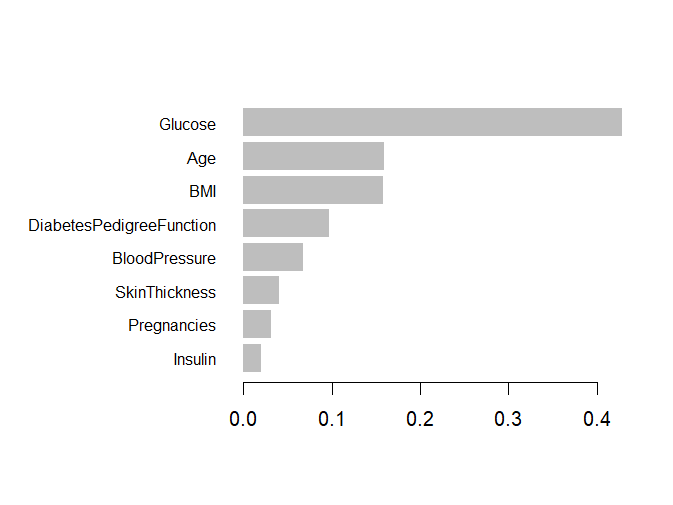
\includegraphics[width=\textwidth]{"C:/Users/msafi/OneDrive/Documents/GitHub/4m_final_project/G1.png"}}
% 		\caption{\centering{Figure 1. ROC Curve for Boosting Model}}
% 		\label{fig:roc}
% 	\end{subfigure}
% 	\hfill
% 	\begin{subfigure}{0.45\textwidth}
% 		\fbox{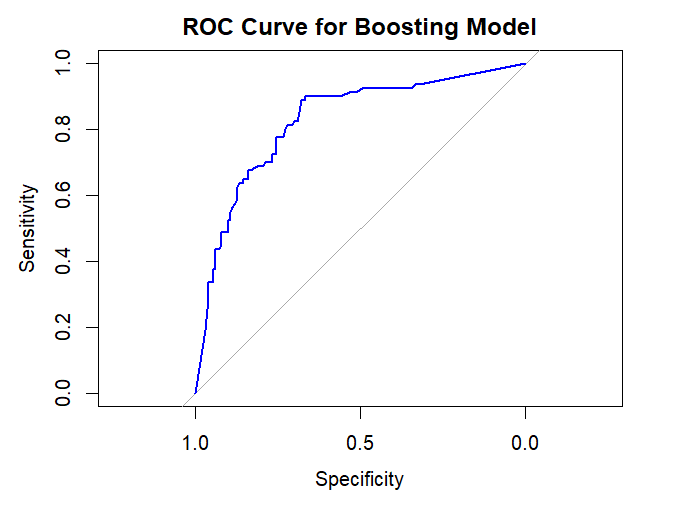
\includegraphics[width=\textwidth]{"C:/Users/msafi/OneDrive/Documents/GitHub/4m_final_project/G2.png"}}
% 		\caption{\centering{Figure 2. Feature Importance Plot}}
% 		\label{fig:importance}
% 	\end{subfigure}
% \end{figure}

Boosting effectively identified significant predictors of diabetes, particularly glucose and BMI. However, the model's performance may be affected by missing data and the dataset's limited size. Future work could address these limitations by imputing missing values and validating the model on larger datasets. Overall, XGBoost proved to be a robust method for this binary classification problem.

\section{Conclusion}

\textbf{TEMPORARY, WILL IMPROVE LATER} Comparison between supervised and unsupervised learning analysis, which method performs better for this dataset, which version of machine learning analysis helps us draw better conclusions for our dataset etc. 

 \section{Bibliography}
 \bibliographystyle{apa} 
 \bibliography{references}

\end{document}

